\documentclass[10pt]{article}
\usepackage{icmlko}

\icmlmeta{IP 파운데이션 월드모델}{154}{낮은 상관, 좁은 오차}{과제 78을 드디어 했다 --- 시장 레코드 51건을 눈가림으로 읽어 매기고 하네스에 심판을 맡겼다. 판 상관은 내려갔는데 오차막대는 3분의 1 줄었다}

\begin{document}

\twocolumn[
\icmlheader

\begin{abstract}
과제 78이 노트 151에서 임계 경로가 됐고 노트 153이 방법을 줬다 ---
\emph{읽는다}. 했다. 유보 구간에 든 시장 레코드 \textbf{51건}을 사람 라벨도
결과값도 안 보고 공유 다섯 축으로 매겼다. 문서 중앙 길이는 158자다(내부
기획서는 676자). 시장 레코드에는 사람이 매긴 축이 없으므로 \textbf{하네스가
심판을 본다}. 결과가 두 갈래로 갈렸고 둘 다 중요하다.
\textbf{① 합치면 내려간다.} 팝업 $\rho$ 가 표준 59에서 $+$0.3505,
축을 비운 116에서 $+$0.3515, \textbf{읽어서 채운 116에서 $+$0.2751}이다.
분모를 두 배로 늘리면 합친 상관은 떨어진다.
\textbf{② 그런데 늘어난 절반 자체는 잡음에서 신호가 됐다.} 노트 151에서
그 절반의 $\rho$ 가 $-$0.085였는데 채우니 \textbf{$+$0.197}이다. 그리고 그
51건만 따로 능형 교차검증하면 \textbf{$+$0.374}다 --- 구조 필드
(\texttt{venue\_type} · \texttt{category})만 쓰면 $+$0.001이므로
\textbf{내가 읽어서 만든 정보가 맞다}. 0.374와 0.197의 차이는 전이 손실이다:
풀링 모형은 내부 레코드로 적합돼 있다.
\textbf{③ 그리고 진짜로 사고 싶었던 것은 상관이 아니라 분해능이었다.}
채운 116으로 재면 팝업 $\rho$ 의 주변 sd 가 0.139에서 \textbf{0.094}로,
정식화 짝 sd 가 0.069$\to$0.059 · 0.034$\to$0.021 · 0.082$\to$0.067로
전부 20$\sim$40\% 준다. \textbf{낮은 상관과 좁은 오차는 다른 것이고, 나는
그 둘을 섞어 부를 뻔했다.} 결론은 분모 규칙(노트 82 · 90)대로다 ---
\textbf{두 분모를 나란히 적는다.} 59는 이력과 견주는 자리, 116은 새 비교를
가르는 자리.
\end{abstract}
]

\begin{figure*}[t]
\centering
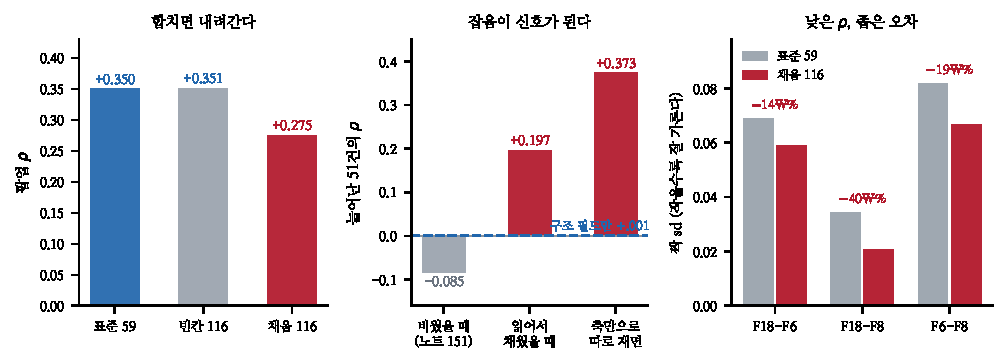
\includegraphics[width=\textwidth]{figs/fill.pdf}
\caption{왼쪽 --- 합치면 내려간다. 가운데 --- 늘어난 절반은 잡음에서
신호가 됐다. 오른쪽 --- 낮은 $\rho$, 좁은 오차.}
\end{figure*}

\section{설계}

노트 151이 잰 대로 유보 116건은 표준 집계 59건과 비표준 57건으로 갈리고,
비표준 쪽은 축이 100\% 비어 있다. 그중 51건이 시장 레코드다. 그 51건의
문서(\texttt{concept\_description} · 체험 요소 · 프로모션 · 장소)만 보고
공유 다섯을 0$\sim$4로 매겼다. 결과값은 안 봤다.

\begin{table}[t]
\centering\tsize
\caption{하네스 심판. F18 배깅 · 씨앗 셋 평균.}
\begin{tabular}{lrrr}
\toprule
& n & 팝업 $\rho$ & 판 $\rho$ \\
\midrule
표준 59 & 59 & $+$.3505 & $+$.4462 \\
빈칸 116 & 116 & $+$.3515 & $+$.4416 \\
\textbf{채움 116} & 116 & \textbf{$+$.2751} & $+$.4385 \\
\bottomrule
\end{tabular}
\end{table}

\claimx{\textbf{합치면 내려간다.} 채워 넣은 116의 팝업 $\rho$ 가 표준
59보다 0.075 낮다. 노트 133에서 능형 태거로 채웠을 때의 붕괴
($+$0.4562$\to$$+$0.1150)보다는 훨씬 얕지만 방향은 같다.}{분모가 다른 두
수를 나란히 놓은 것이므로 이것만으로 ``나빠졌다''고 하면 안 된다 ---
노트 82 · 90의 분모 규칙이 정확히 이 자리를 막는다.}

\section{늘어난 절반은 잡음에서 신호가 됐다}

\begin{table}[t]
\centering\tsize
\caption{늘어난 51건만 따로.}
\begin{tabular}{lrl}
\toprule
& $\rho$ & \\
\midrule
축을 비웠을 때 (노트 151) & $-$.085 & 잡음 \\
\textbf{읽어서 채웠을 때} & \textbf{$+$.197} & 하네스 안 \\
\textbf{축만으로 따로 재면} & \textbf{$+$.374} & 능형 5겹 \\
\midrule
구조 필드만 (venue\_type · category) & $+$.001 & \\
\bottomrule
\end{tabular}
\end{table}

\claimx{\textbf{읽어서 만든 정보가 맞다.} 같은 51건에서 구조 필드
(장소 유형 5종 · 카테고리 9종)만 쓰면 $\rho$ 가 $+$0.001이고 내가 매긴 다섯
축만 쓰면 $+$0.374다. \textbf{문서에 이미 적혀 있던 것을 다시 부호화한 것이
아니다.}}{$n{=}51$ 이라 $\rho$ 의 표준오차가 0.14쯤이다. $+$0.374와
$+$0.001은 그 폭으로 안 겹친다.}

\claimx{\textbf{0.374와 0.197의 차이는 전이 손실이다.} 축 자체는 0.374를
품고 있는데 하네스 안에서는 0.197만 나온다. 풀링 모형이 \emph{내부
레코드}로 적합돼 있고, 내부 기획서(676자)와 시장 기사(158자)에서 매긴 축은
눈금이 다르기 때문이다.}{과제 78이 물은 ``전이 오차''가 이 값이다 ---
절반 가까이(47\%) 잃는다. 없애는 길은 시장 레코드를 학습에도 넣는 것인데,
그러면 학습 분포가 바뀌므로 따로 재야 한다.}

\section{그런데 사려던 것은 상관이 아니라 분해능이었다}

\begin{table}[t]
\centering\tsize
\caption{팝업 유보에서 정식화 둘을 가르는 데 드는 오차. 재추출 400.}
\begin{tabular}{lrrr}
\toprule
& 표준 59 & \textbf{채움 116} & 줄어든 폭 \\
\midrule
주변 sd (F18) & .1391 & \textbf{.0940} & $-$32\% \\
F18$-$F6 & .0689 & \textbf{.0591} & $-$14\% \\
F18$-$F8 & .0344 & \textbf{.0206} & $-$40\% \\
F6$-$F8 & .0819 & \textbf{.0667} & $-$19\% \\
\bottomrule
\end{tabular}
\end{table}

\claimx{\textbf{오차막대가 전부 줄어든다.} 상관은 내려갔는데 가르는 힘은
세졌다. \textbf{둘은 다른 것이다} --- $\rho$ 는 ``얼마나 잘 맞히나''이고
sd 는 ``두 방법의 차이를 볼 수 있나''다. 팝업 59건에서 아무것도 못 갈랐던
이유가 후자였다(노트 148).}{점 추정이 뒤집히는 짝이 있다 --- F18$-$F6 이
$-$0.041에서 $+$0.042로, F6$-$F8 이 $+$0.039에서 $-$0.012로. 둘 다 오차
안이라 모순은 아니지만, \textbf{새 표본의 순서를 채택하지는 않는다}
(노트 133).}

\section{그래서 분모를 둘 적는다}

\begin{table}[t]
\centering\tsize
\caption{어느 자리에 어느 분모를 쓰나.}
\begin{tabular}{ll}
\toprule
\textbf{59 (표준 집계)} & 노트 132 이후의 이력과 견줄 때 \\
\textbf{116 (읽어서 채움)} & 새 정식화 · 새 축을 가를 때 \\
\bottomrule
\end{tabular}
\end{table}

노트 82 · 90의 분모 규칙은 ``대상 집합이 기준과 같아야 비교가 성립한다''
였다. 여기서는 두 집합이 각각 잘하는 일이 다르므로 하나를 고르는 대신
둘 다 적는다. \textbf{섞어서 한 줄로 쓰면 그때 규칙이 깨진다.}

\begin{table}[t]
\centering\tsize
\caption{남은 것.}
\begin{tabular}{ll}
\toprule
전이 손실 & 0.374$\to$0.197 --- 시장 레코드를 학습에도 넣으면 \\
남은 57 & 학습 구간의 빈칸도 채우면 학습이 두 배 \\
눈금 & 158자와 676자에서 매긴 축의 눈금이 다르다 \\
\bottomrule
\end{tabular}
\end{table}

첫 줄이 다음이다. 지금은 시장 레코드를 \emph{채점}에만 넣었다. 학습에도
넣으면 풀링 모형이 그 눈금을 배울 수 있고, 전이 손실 47\%의 상당 부분이
거기서 온다면 회수된다. 다만 학습 분포를 바꾸는 결정이라 노트 82의 규칙에
따라 자료 결정으로 미리 적어 두고 재야 한다.

\end{document}
